%!TEX encoding = UTF-8 

\chapter{Experimental Results}
\label{chap:experimental_results}

This chapter contains experimental results obtained by testing the programs that were written for this thesis. The whole project was carried out at Computer and Robot Vision Laboratory~\cite{link:vislab}, Institute for Systems and Robotics, Instituto Superior T\'{e}cnico, Lisbon (Portugal) for eight months during 2008.

All the tests were performed on the machine that is attached to the Baltazar\index{Baltazar} robotic platform: a personal computer with a Dual Intel Xeon 3.20GHz processor, 1GB of RAM, running Microsoft Windows XP Pro SP2.

The development environment adopted was Microsoft Visual Studio 2005, also providing a graphical debugging interface for C++.

%%%%%%%%%%%%%%%%%%%
%%%%%%%%%%%%%%%%%%%
\section{Segmentation and Tracking}

\begin{figure}[h]
\centering
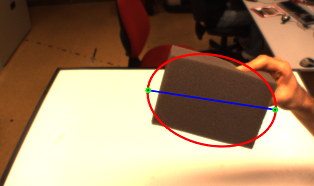
\includegraphics{figures/0619grey}
\caption[\acs{CAMSHIFT} tracking experiment]{\ac{CAMSHIFT} tracking experiment, with a grey sponge.}
\label{img:0619grey}
\end{figure}

Fig.~\ref{img:0619grey} shows an early version of the custom modified \ac{CAMSHIFT}\index{CAMSHIFT} tracker while running during a video experiment. The best-fit enclosing ellipse is drawn in red, the major axis in blue.

The major axis of the ellipse\index{ellipse} represents an estimation of the target object orientation. One can see that such axis is not completely parallel to the long edges of the cuboid sponge: this is due to previous motion and frames that cause an oscillatory nature of the ellipse (axes).

Furthermore, we can see the estimated extremities of the major axis ($p_1$ and $p_2$) marked with green circles. Note that this type of experiments did not yet take into account the manipulation (reaching and grasping) of objects, thus the object centroid is neither estimated nor visually marked.

All in all, this first experiment (which involved only one instance of \ac{CAMSHIFT}\index{CAMSHIFT} tracker running at a time---no stereo vision yet) proved quite successful. The tracked object, a grey sponge, was tracked continuously for several minutes. When the object was shaken (rotated) very fast in the experimenter's hand, it was still tracked. This means that each iteration of \ac{CAMSHIFT} managed to use the colour histogram successfully for its search. On the other hand, there were some stability issues with the major ellipse of the axis or when the object was occluded for a few seconds (the tracker would not completely lose it, but its tracked region would shrink to the very small visible portion of the sponge during the occluded sequence, predictably making the axis shake between various orientations).



\begin{figure}
\centering
\subfloat[][Second \ac{CAMSHIFT} tracking experiment screenshot.]
{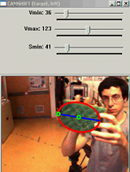
\includegraphics[width=.40\columnwidth]{figures/1225camshift_green} \label{img:1225camshift_green} } \quad
% %necessary to prevent line break
\subfloat[][16-bin \ac{CAMSHIFT} colour histogram used for iterative searches during all of the experiment of Fig~\ref{img:1225camshift_green}.]
{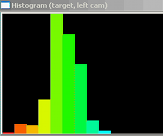
\includegraphics[width=.50\columnwidth]{figures/1225histo} \label{img:1225histo} }
%
\caption[Second \acs{CAMSHIFT} tracking experiment]{Another \ac{CAMSHIFT} tracking experiment, with a green sponge.}
\label{img:1225camshift_exp}
\end{figure}

Fig.~\ref{img:1225camshift_exp} shows the execution of another \ac{CAMSHIFT} tracking task. Here, we are computing (and displaying) not the reconstructed extremities $p_1$ and $p_2$ of the major axis of the ellipse\index{ellipse}, but rather $p_1$ and the estimated object centroid. Fig.~\ref{img:1225histo} shows the 16-bin colour histogram after it has been initialized for this experiment (green is the colour the tracker will look for, at every iteration). Note that the histogram remains constant during the whole experiment, also providing some robustness against occlusions\index{occlusion}.


%%%%%%%%%%%%%%
%%%%%%%%%%%%%%
\section{3D Reconstruction}
\index{3D reconstruction}\index{stereopsis}

\begin{figure}[h]
\centering
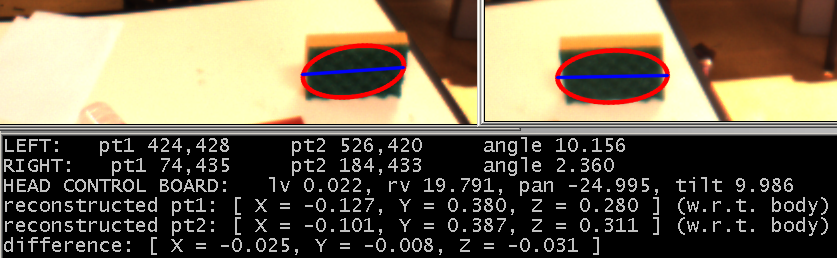
\includegraphics[scale=0.4]{figures/0509recon}
\caption[3D reconstruction experiment]{3D reconstruction experiment.}
\label{img:0509recon}
\end{figure}

In Fig.~\ref{img:0509recon} we can see the output of the 3D reconstruction module during an experiment. Three windows are visible:
\begin{itemize}
\item left eye \ac{CAMSHIFT} tracker;

\item right eye \ac{CAMSHIFT} tracker; and

\item 3D reconstruction module output.
\end{itemize}

As far as the two trackers are concerned, we can see an optimal behaviour and drawing of the ellipses with their respective major axes. This contrasts with previous tracking experiments such as Fig.~\ref{img:0619grey} for a number of reasons: first of all, the tracked sponge is not moving now. Because we were interested in measuring and judging the quality of our 3D reconstruction\index{3D reconstruction}, in this experiment we chose a static scenario (there was some minor flickering and oscillation in the camera views during the video, but it was a negligible phenomenon, as the tracked axis kept stable throughout the whole experiment). Secondly, the tracked object was completely in front of the white table that is in front of Baltazar\index{Baltazar}---greatly facilitating colour segmentation\index{image segmentation}.

The most important part of this experiment, though, is the behaviour of the 3D reconstruction\index{3D reconstruction} module. It is the black window with white text at the bottom of Fig.~\ref{img:0509recon}. The first three lines of text, written in capital letters, contain numerical values used internally by the 3D reconstruction module: coordinates in pixels, angles in degrees and lengths in metres. Then, the coordinates of the two extremities of the reconstructed axis ($p_1$ and $p_2$) are printed, in a $(X, Y, Z)$ world reference frame, where $Z$ is positive in the direction in front of the face of Baltazar. This means, for example, that a coordinate of
\[
Z = 0.280
\]
(metres) corresponds to 28 cm in front of the robot torso, on the white table.

The 3D reconstructed coordinates are correct in this experiment: they were checked with a ruler and the error along all the three dimensions was small (less than 5 cm).

Finally, the orientation of the target object (encoded as the different between reconstructed $p_1$ and reconstructed $p_2$) is printed.



% Paulo's:
%\begin{figure}
%\centering
%\subfloat[][$x$ error.]
%{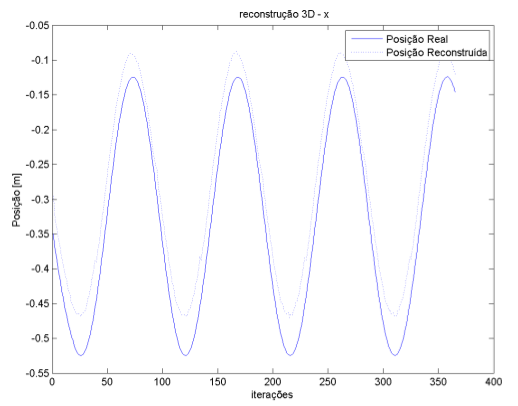
\includegraphics[width=.70\columnwidth]{figures/recon_error_x} \label{fig:recon_error_x} } \\
%\subfloat[][$y$ error.]
%{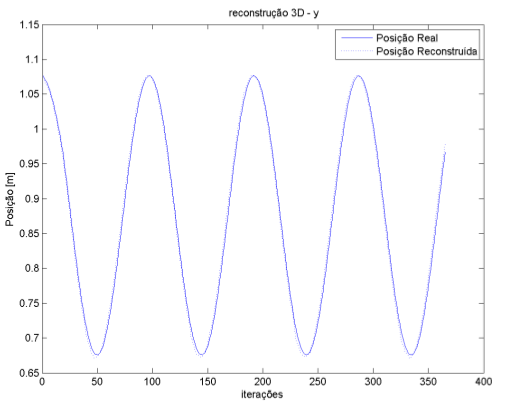
\includegraphics[width=.70\columnwidth]{figures/recon_error_y} \label{fig:recon_error_y} } \\
%\subfloat[][$z$ error.]
%{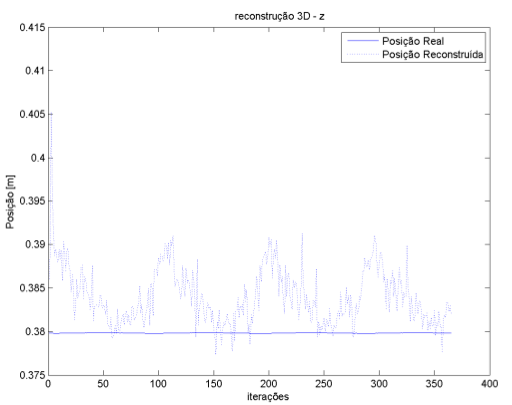
\includegraphics[width=.70\columnwidth]{figures/recon_error_z} \label{fig:recon_error_z} }
%
%\caption[3D reconstruction error during tracking]{3D reconstruction error while tracking a moving object.}
%\label{fig:recon_error}
%\end{figure}





%%%%%%%%%%%%%%%%%%%
%%%%%%%%%%%%%%%%%%%
\section{Object Manipulation Tasks}
\index{manipulation}

%%%%%%%%%%%%%%%%%%
\subsection{Reaching Preparation}
\index{reaching}

\begin{figure}[h]
\centering
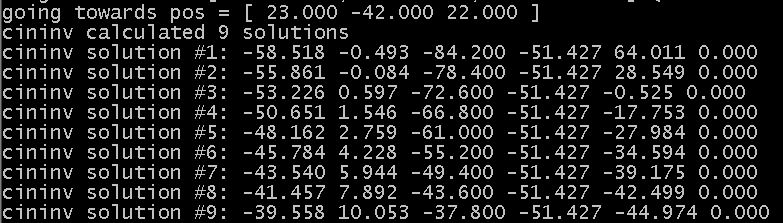
\includegraphics[scale=0.5]{figures/10xxcininv}
\caption[Object manipulation: inverse kinematics experiment]{Object manipulation: inverse kinematics solver experiment.}
\label{img:10xxcininv}
\end{figure}

Recall (p.~\pageref{intro:reaching_phases}) that in accordance to our perceptual framework we have split the reaching task in two distinct phases:
\begin{description}
\item[reaching preparation:] an open-loop ballistic phase to bring the manipulator to the vicinity of the target, whenever the robot hand is not visible in the robot's cameras;

\item[grasping preparation:] a closed-loop visually controlled phase to accomplish the final alignment to the grasping position.
\end{description}

We shall now focus on the first problem, reaching preparation. In this phase our aim is to position the anthropomorphic arm of Baltazar, initially outside of the cameras' field of view, in the ``vicinity'' of the target. To start off, we define this vicinity as the 3D reconstructed coordinates of the centroid of the target object, minus a safety threshold of 20 cm along the horizontal axis (parallel to the table and to the ground, directed towards the right of the robot, from its own point of view). So, for this phase to be successful, we need to position the robot wrist at 20 cm from the object centroid. A necessary condition to accomplish this, is to solve the robot arm inverse kinematics for the desired hand position coordinates.

Fig~\ref{img:10xxcininv} shows a number of inverse kinematics solutions found for Cartesian coordinates
\[
X = 23, Y = -42, Z = 22 \quad \textrm{[cm]}.
\]

Specifically, each of the 9 inverse kinematics solutions is a vector of 6 joint angles $\mathbf{q} = [q_1, q_2, q_3, q_4, q_5, q_6]$, expressed in degrees. The 6 angles correspond to the 6 encoder values that are actually streamed by the \ac{YARP} arm server of Baltazar (see Table~\ref{tab:balt_arm_joints}). Upon inspection of the computed results, two things immediately strike one's attention:
\begin{itemize}
\item $q_4$ (elbow) has the same constant value ($-51.427 \degree\!$) for all the solutions;

\item $q_6$ (wrist) is constantly zero.
\end{itemize}

The output of the fourth column, $q_4$, has always the same value because there exists a redundancy between this joint and the hand ones (several possible inverse kinematics solutions, depending on how ``high'' the elbow is). In particular, these joints only affect the orientation of the \emph{hand}, so we applied a simplification here, to reduce the number of solutions. Also, recall that the end-effector of Baltazar is designed to be the base of the wrist (p.~\pageref{balta_ee}), not the palm of the hand or the tip of any finger.

\begin{figure}
\centering
\subfloat[][Arm is at a predefined position out of the robot field of view.]
{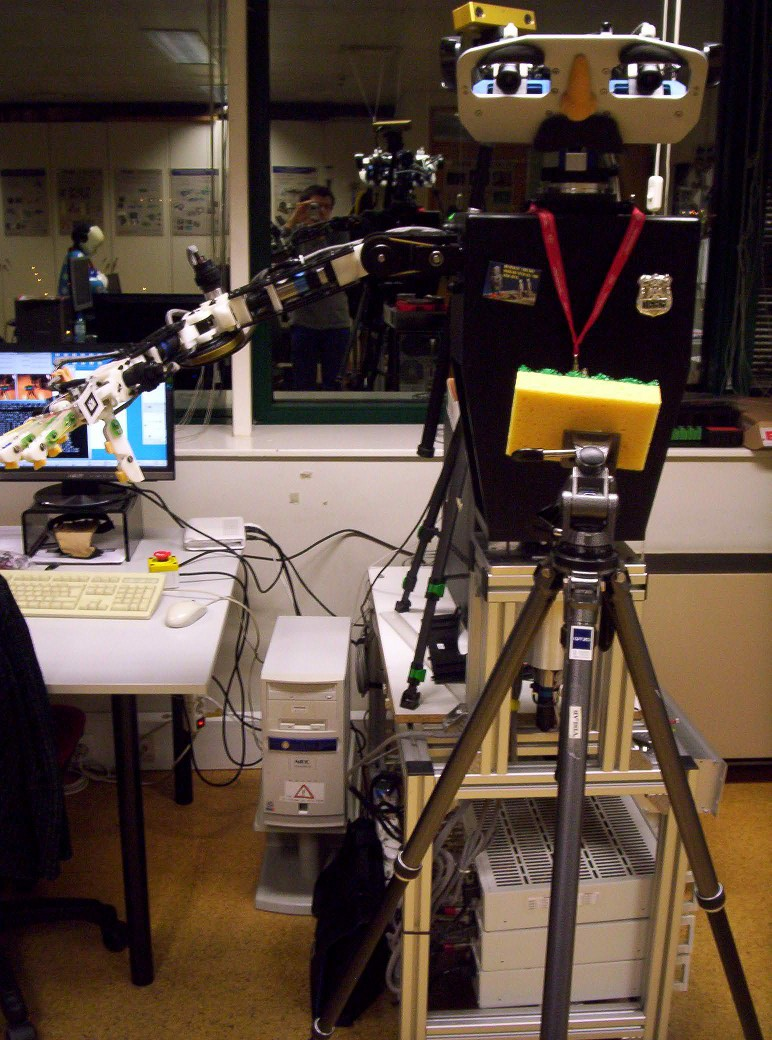
\includegraphics[width=.45\columnwidth]{figures/1106reach1} \label{img:1106reach1} } \quad
% %necessary to prevent line break
\subfloat[][Robot arm is now within the field of view of cameras.]
{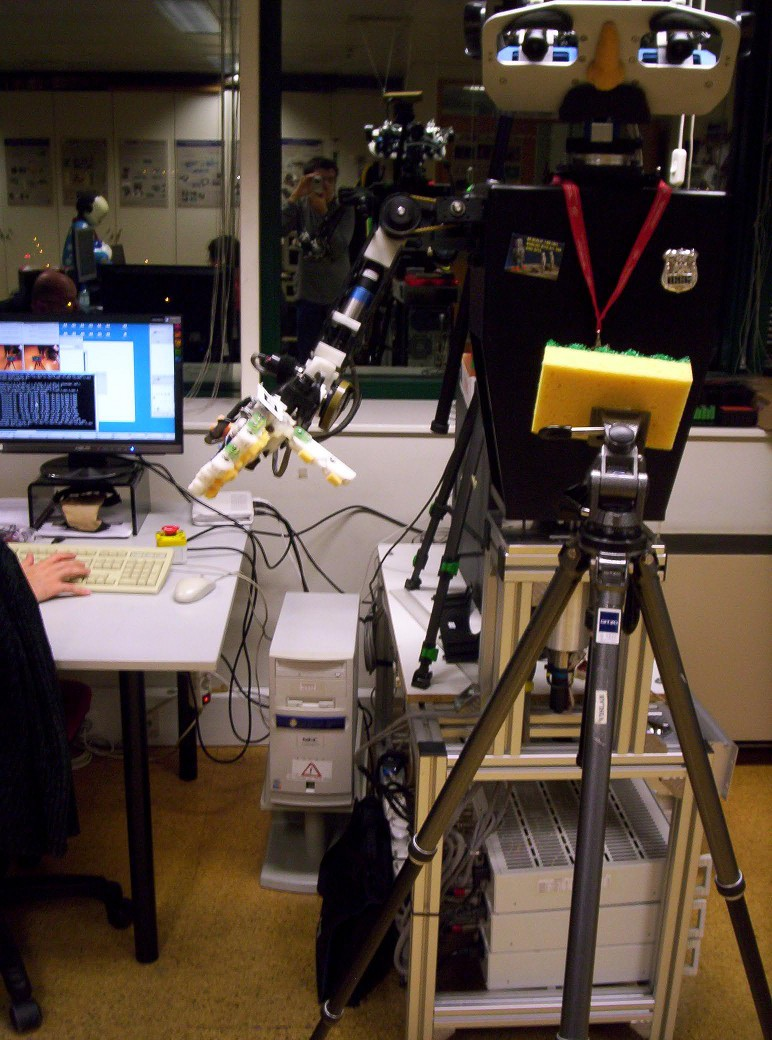
\includegraphics[width=.45\columnwidth]{figures/1106reach2} \label{img:1106reach2} } \\
\subfloat[][Hand is finally positioned at target (minus a safety horizontal threshold).]
{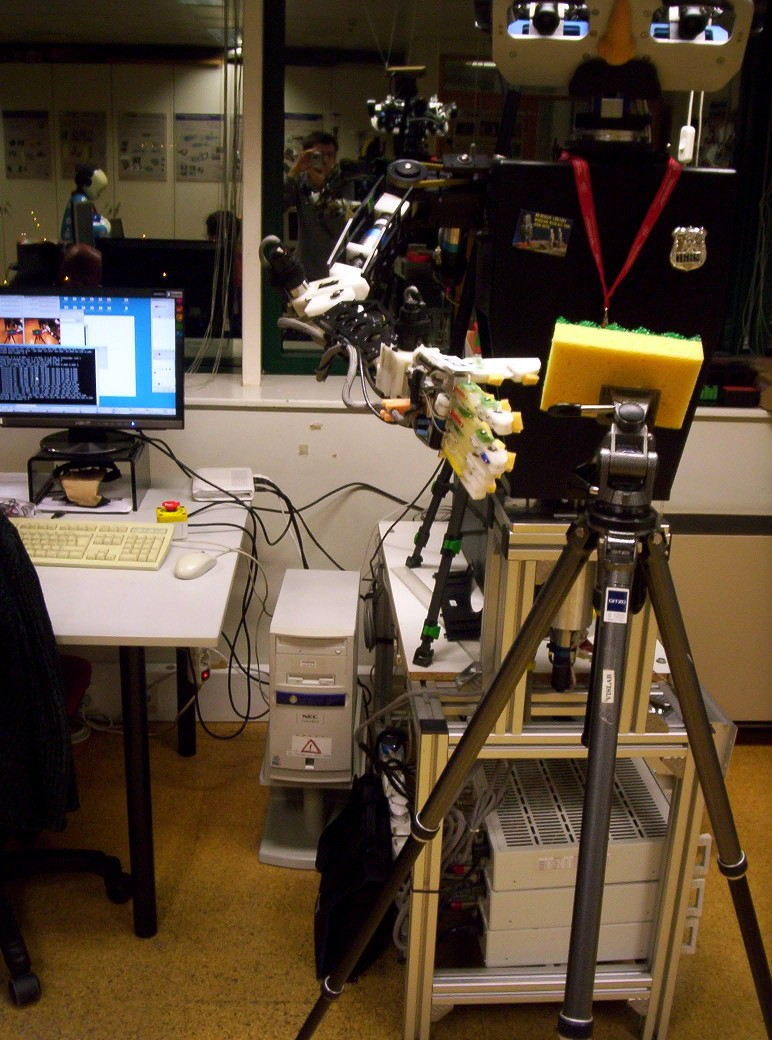
\includegraphics[width=.45\columnwidth]{figures/1106reach3} \label{img:1106reach3} }

\caption[Reaching preparation experiment]{Reaching preparation task experiment: the robot arm moves gradually towards the estimated centroid position of the target object.}
\label{img:1106reach}
\end{figure}

Moving on from inverse kinematics to actual arm actuating, Fig.~\ref{img:1106reach} shows an experiment of a reaching preparation task. Initially (Fig.~\ref{img:1106reach1}) the arm is positioned outside of the robot cameras' field of view, at a predefined position. Then it is moved within the field of view. Finally (Fig.~\ref{img:1106reach3}), the robot arm is correctly positioned in the vicinity of the 3D estimated object centroid coordinates, within a safety threshold of 20 cm from it.

%%%%%%%%%%%%%%%%%%
\subsection{Grasping Preparation}
\index{grasping}

The second and last phase of the reaching task is the ``grasping preparation'' phase. Contrary to reaching preparation, this task uses closed-loop feedback control. At the beginning of this task, hand and target object are already quite close (for example at a distance of 20 cm, in accordance to the desired safety threshold that we have imposed during the previous phase). The objective of grasping preparation is a more precise alignment of hand and target, thanks to a control law.

At the time of writing this thesis, experiments for this section were still at an initial stage. However, we did test the necessary arm control law\index{control law} computations and show here some results.

\begin{figure}
\centering
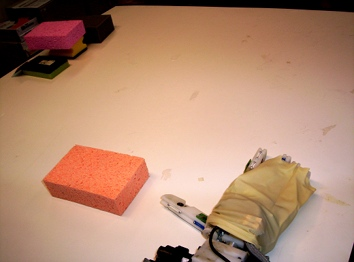
\includegraphics{figures/0619glove}
\caption[Robot hand wearing a glove]{Baltazar robot hand wearing a glove, in order to make its colour more homogeneous, thus facilitating \acs{CAMSHIFT} tracking and 3D reconstruction of the hand.}
\label{img:0619glove}
\end{figure}

Fig~\ref{img:0619glove} shows the hand of Baltazar\index{Baltazar} wearing a latex glove in the vicinity of the target object. We applied this glove in an attempt to make colour segmentation (of the hand) more robust, thanks to a more uniform colour to be found by the search histogram of \ac{CAMSHIFT}. This glove does not impede finger movement, so it is not a problem for the grasping itself.


\begin{figure}
\centering
\subfloat[][Object and hand are parallel; $\mathbf{u} = (X = -0.006, Y = -0.062, Z = -0.041), \theta = 4.285\degree$.]
{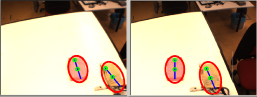
\includegraphics[width=.9\columnwidth]{figures/angle04small} \label{fig:angle04} } \\

\subfloat[][Object and hand have a relative slope of roughly $45\degree$; $\mathbf{u} = (X = -0.129, Y = 0.737, Z = -0.129), \theta = 49.413\degree$.]
{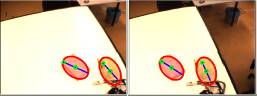
\includegraphics[width=.9\columnwidth]{figures/angle49small} \label{fig:angle49} } \\

\subfloat[][Orthogonality scenario; $\mathbf{u} = (X = -0.146, Y = 0.919, Z = 0.362), \theta = 87.408\degree$.]
{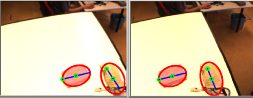
\includegraphics[width=.9\columnwidth]{figures/angle87small} \label{fig:angle87} }

\caption[Evaluation of target--hand axis and angle]{Evaluated axis $\mathbf{u}$ and angle $\theta$ between tracked object and hand in several scenarios in three different stereo pairs.} \index{angle--axis parameterization}
\label{img:angles}
\end{figure}

Fig.~\ref{img:angles} displays some tests done when tracking and 3D reconstructing\index{3D reconstruction} both a target object and a robot hand at the same time. The relative angle--axis alignment is thus computed, as per Eq.~\ref{eq:cross_prod}. The initial results on this part are promising, as the three obtained angle values are similar to the real ones: 0, 45, 90 degrees, respectively.